% Extensión estimada: unas 6 páginas, dos subsecciones, una tabla y dos figuras (ficha 5.3).
% Fuentes: cap5_derivados.json ("ruteo"), ensemble_bootstrap{,_llava_med}_les_report_only_strict.json
% ("tab_incertidumbre_e2e"), uncertainty_analysis{,_llava_med}_les.json (taxonomía por nivel, abstenidas);
% Codigo/docs/ejecuciones.md, 18/10/2026 (bloques <think> sin cerrar de LLaVA-Med en el diferencial: 144 de 248).
% Cohorte completa: aciertos del pipeline (0.901 × 1 452 = 1 308; LLaVA-Med 0.744 × 1 452 = 1 080) sobre 1 503.
% Figuras: scripts/figuras_cap5.py (ruteo-niveles); ejemplos-reportes.tex.
% Revisión del tutor del 26/10/2026: el ruteo se nombra con su referencia al Capítulo 3 sin volver a describirlo;
% esquema contexto → objeto → valores → conjetura.
\section{Pipeline completo}
\label{sec:res_gen_incertidumbre}

En la cascada, el reporte suele afirmar el diagnóstico del clasificador, aunque sea incorrecto, y ni la imagen ni los vecinos lo corrigen en la mayoría de los casos. El último paso del recorrido agrega el ruteo por concordancia de la Sección~\ref{sec:met_ruteo}, que
completa el \emph{pipeline} de la Figura~\ref{fig:met_pipeline} del Capítulo~\ref{cp:metodos}: según coincidan o no
Swin-Tiny y el \gls{knn}, cada imagen recibe un reporte afirmativo, un reporte diferencial con dos candidatos o se
deriva a un especialista, según los tres niveles de la Tabla~\ref{tab:met_niveles} del Capítulo~\ref{cp:metodos}.

Esta sección presenta los resultados del ruteo en dos partes. La primera evalúa si la concordancia separa los casos en
que el clasificador acierta de aquellos en que se equivoca. La segunda mide cuánto cambian los reportes de Mini-VLM y
LLaVA-Med frente a la cascada simple de la sección anterior y a la línea base sin generador de la
Sección~\ref{sec:met_referencias}.

\subsection{Concordancia entre el clasificador y el kNN}
\label{sec:res_gen_concordancia}

El ruteo asigna ocho de cada diez imágenes del conjunto de prueba al nivel afirmativo, una de cada seis al diferencial y una
de cada treinta a la derivación. Para ver si esos niveles reúnen casos de dificultad distinta, la Figura~\ref{fig:res_gen_ruteo} presenta dos paneles. El
panel (a) indica, en cada nivel, la fracción de casos en que Swin-Tiny acierta y en que el par de candidatos contiene la
clase verdadera. El panel (b) reparte las imágenes de cada clase entre los tres niveles.

\begin{figure}[H]
    \centering
    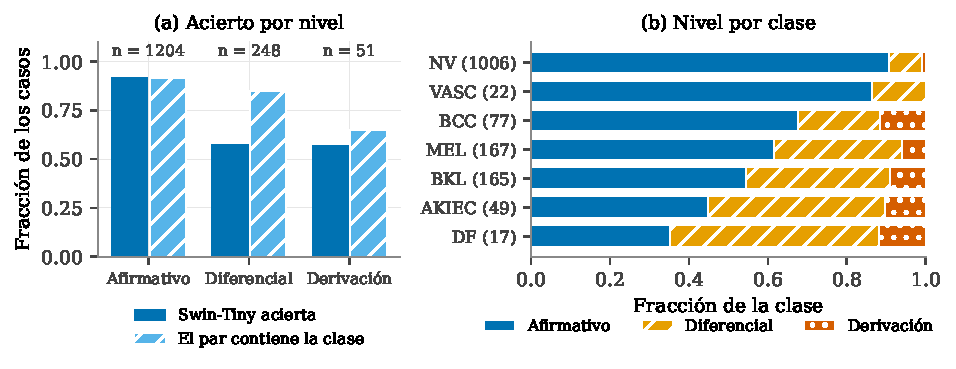
\includegraphics[width=\textwidth]{Figures/Capitulos/05-Resultados-Generacion/ruteo-niveles.pdf}
    \caption{(a) Acierto de Swin-Tiny y del par de candidatos en cada nivel del ruteo; (b) nivel asignado a las
    imágenes de cada clase, con el número de imágenes entre paréntesis.}
    \label{fig:res_gen_ruteo}
\end{figure}

Swin-Tiny acierta el 91.5\,\% de los casos afirmativos y poco más de la mitad de los otros dos niveles. En este conjunto de prueba, la concordancia discrimina subconjuntos con diferentes tasas de error, como suponía el diseño del ruteo (Sección~\ref{sec:met_ruteo}), y su transferencia a otros conjuntos debe evaluarse aparte. Tampoco proporciona una estimación calibrada de confianza para cada caso.

En el nivel diferencial, presentar los dos candidatos cubre muchos más casos que el diagnóstico del clasificador
solo. El par formado por la clase de Swin-Tiny y el voto del \gls{knn} contiene la clase verdadera en el 84.7\,\% de
esos casos, frente al 57.3\,\% del clasificador. El voto del \gls{knn} acierta en ellos con menos frecuencia que
Swin-Tiny, pero, como en este nivel los dos predictores difieren, cada acierto del \gls{knn} corresponde a un error
del clasificador, y eso es lo que justifica usarlo como segunda opinión.

La concordancia, sin embargo, no detecta los errores que comparten ambos predictores. De los 230 casos en que
Swin-Tiny se equivoca, 102 caen en el nivel afirmativo, porque el \gls{knn} vota la misma clase errónea. Es decir,
cuatro de cada nueve errores del clasificador se afirman con la misma plantilla que un acierto, la limitación que
anticipaba la Sección~\ref{sec:met_ruteo}. El caso más relevante es el melanoma: 38 de los 167 melanomas del conjunto de prueba
se afirman como otra clase, 31 de ellos como \gls{nv}, de modo que casi uno de cada cuatro melanomas recibe un
reporte definitivo con un diagnóstico benigno.

Por clase, el panel (b) muestra que el ruteo afirma casi todos los \gls{nv} y las lesiones vasculares, y deriva o
presenta como diferencial más de la mitad de las imágenes de \gls{df} y de \gls{akiec}. El melanoma queda en una
posición intermedia. Un tercio de los melanomas va al nivel diferencial, y en ese caso el par de candidatos contiene el
melanoma en 52 de 54 imágenes, la mayoría como par melanoma--nevo, la confusión más costosa según la
Sección~\ref{sec:met_seleccion}.

La derivación, por último, deja fuera del \emph{pipeline} 51 casos en los que el clasificador acierta tan poco como en
el nivel diferencial. Esta decisión tiene un costo: en esos casos, con la cascada simple, Mini-VLM habría escrito 20
reportes con un diagnóstico incorrecto y dos con una contradicción, mientras que el clasificador acierta 29 de los 51
diagnósticos, que la derivación también descarta. Por eso la derivación evita errores y deja sin reporte 29 diagnósticos correctos, y su utilidad depende de cuánto cueste en la práctica un error frente a una consulta con el
especialista.

\subsection{Reportes del pipeline completo}
\label{sec:res_gen_pipeline}

Con el ruteo, los casos afirmativos reciben el reporte de la cascada y los diferenciales, uno que discute los dos
candidatos. La Tabla~\ref{tab:res_gen_pipeline} compara la consistencia de esos reportes, para Mini-VLM y LLaVA-Med
(columnas), en tres bloques de filas. El primero reúne los 1\,452 casos no derivados, con la cascada simple, el
\emph{pipeline}, la línea base sin generador, que escribe el diagnóstico afirmado o el par de candidatos, y las
diferencias pareadas con su intervalo de confianza. El segundo se limita al nivel diferencial, y el tercero vuelve al conjunto de prueba completo, con cada derivación contada como un caso sin diagnóstico.

Esta consistencia no equivale a una exactitud, por dos razones. Primero, en el nivel diferencial un reporte que nombra
dos candidatos cuenta como consistente si uno de ellos es el verdadero, de modo que el criterio se parece a acertar
entre las dos primeras opciones. Segundo, la consistencia de los casos no derivados excluye las derivaciones, que son
de los más difíciles, y por eso el tercer bloque informa también la consistencia sobre las 1\,503 imágenes.

\begin{table}[H]
    \centering
    \caption{Consistencia diagnóstica del pipeline completo frente a la cascada simple y a la línea base sin
    generador. Entre corchetes, el intervalo de confianza (IC) del 95\,\% de cada diferencia, estimado con \emph{bootstrap} pareado (Sección~\ref{sec:met_estadistica}); una diferencia cuyo IC no incluye el cero es estadísticamente significativa. En negrita, el mayor valor de cada bloque y las diferencias cuyo IC no incluye el cero.}
    \label{tab:res_gen_pipeline}
    \small
    \setlength{\tabcolsep}{4pt}
    \begin{tabularx}{\textwidth}{@{}>{\raggedright\arraybackslash}X cc@{}}
        \toprule
        & \textbf{Mini-VLM} & \textbf{LLaVA-Med} \\
        \midrule
        \multicolumn{3}{@{}l}{\textit{Casos no derivados (1\,452)}} \\
        Cascada simple & 0.858 & 0.755 \\
        Pipeline completo & 0.901 & 0.744 \\
        Línea base sin generador & \textbf{0.904} & \textbf{0.904} \\
        Pipeline $-$ cascada simple & $\mathbf{+0.043}$ [$+0.031$, $+0.055$] & $-0.011$ [$-0.025$, $+0.003$] \\
        Pipeline $-$ línea base sin generador & $-0.003$ [$-0.008$, $+0.002$] & $\mathbf{-0.160}$ [$-0.180$, $-0.140$] \\
        \filasep
        \multicolumn{3}{@{}l}{\textit{Nivel diferencial (248)}} \\
        Cascada simple & 0.581 & 0.472 \\
        Reporte diferencial & 0.831 & 0.407 \\
        Par de candidatos, sin generador & \textbf{0.847} & \textbf{0.847} \\
        \filasep
        \multicolumn{3}{@{}l}{\textit{Conjunto de prueba completo, con las derivaciones sin diagnóstico (1\,503)}} \\
        Cascada simple & 0.849 & 0.745 \\
        Pipeline completo & 0.870 & 0.719 \\
        Línea base sin generador & \textbf{0.873} & \textbf{0.873} \\
        \bottomrule
    \end{tabularx}
\end{table}

La línea base sin generador obtiene la consistencia más alta en los tres bloques, y LLaVA-Med en el \emph{pipeline},
la más baja. Con Mini-VLM, el \emph{pipeline} obtiene una mayor consistencia diagnóstica que la cascada simple según la métrica utilizada. Esta mejora se concentra en el nivel diferencial, donde el reporte nombra la clase verdadera en cuatro de cada cinco casos, frente a seis de cada diez de la cascada. En ese nivel se consideran consistentes los reportes que incluyen la clase verdadera entre dos candidatos, por lo que la mejora no equivale directamente a un aumento de la exactitud diagnóstica. Sin embargo, el \emph{pipeline} no supera a la línea base sin generador. La ganancia puede atribuirse, por lo tanto, a presentar dos candidatos cuando los predictores discrepan, una decisión del ruteo, y el generador la
conserva sin agregarle fidelidad. Sobre el conjunto de prueba completo, con las derivaciones contadas como casos sin diagnóstico,
la mejora es menor, de 0.849 a 0.870. Esta lectura coincide con la de la cascada: el diagnóstico sale de los
predictores, y el generador lo redacta.

Con LLaVA-Med, en cambio, el \emph{pipeline} no mejora la cascada simple, y sobre el conjunto de prueba completo queda por debajo de
ella. Sus reportes diferenciales nombran la clase verdadera en cuatro de cada diez casos, la mitad que el par de
candidatos que reciben. En 144 de los 248, el generador abre un bloque de razonamiento que el límite de tokens deja sin
cerrar, y los candidatos quedan dentro de él. Como la evaluación mide solo el reporte
(Sección~\ref{sec:met_eval_generacion}), esos candidatos no cuentan. Una explicación posible es que la plantilla
diferencial, que pide discutir dos candidatos, induce a LLaVA-Med a razonar, mientras que la plantilla
\emph{noreasoning} del nivel afirmativo lo evita en general.

Según la clasificación de fallas de la Sección~\ref{sec:res_gen_errores}, disminuye también la proporción de reportes con un diagnóstico incorrecto, es decir, que nombran otra clase y no la verdadera. Entre los 1\,452 casos no derivados, bajan del 13.6\,\% al 9.0\,\% con Mini-VLM y del 9.4\,\% al 7.1\,\% con LLaVA-Med, si en el nivel diferencial se cuenta como
correcto el reporte que incluye la clase verdadera entre los dos candidatos. Esta reducción refleja en parte la presentación de diagnósticos alternativos y no debe interpretarse directamente como una disminución equivalente del riesgo clínico. El precio es un formato menos estable, ya que
los reportes diferenciales de Mini-VLM nombran en promedio más de dos clases y los reportes con repeticiones internas pasan de 7 a 48 de los 1\,452 casos no derivados.

Las métricas anteriores no muestran cómo se lee un reporte. Para completarlas con un análisis cualitativo, la
Figura~\ref{fig:res_gen_ejemplos} reúne tres reportes de
Mini-VLM en el \emph{pipeline}, uno por situación, citados en inglés. En el primero, el clasificador y los vecinos coinciden en
melanoma, y el reporte afirma el diagnóstico de melanoma y menciona características habitualmente asociadas con esa categoría, como bordes irregulares y asimetría.

El segundo es un caso diferencial: el clasificador predice melanoma, dos de los tres vecinos son nevos, y el reporte
discute los dos candidatos y recomienda una biopsia. El texto incluye, sin embargo, una oración que repite la
instrucción recibida («The final clinical report should include…»), un defecto de redacción que las métricas
automáticas no detectan. El tercero es un error compartido: el clasificador y los tres vecinos coinciden en nevo para
un melanoma, y el reporte afirma el nevo y describe una pigmentación homogénea «with no visible melanocytic infiltration or atypical features». Es decir, la
descripción acompaña al diagnóstico recibido, y un error del clasificador llega al reporte con rasgos que lo hacen
verosímil.

En conjunto, el ruteo identifica una parte de los casos dudosos y, en ellos, presentar dos candidatos cubre más que
afirmar uno, aunque los errores compartidos por los dos predictores se siguen afirmando. La sección siguiente compara
los tres generadores con estos resultados y con su costo de ejecución.

% Tres reportes reales de Mini-VLM (configuración principal), elegidos con scripts de lectura sobre
% outputs/generated_reports/mini_vlm/{full_swin_les,full_differential_les}: el nivel afirmativo con el diagnóstico
% correcto, el diferencial con el par {Swin-Tiny, kNN} y el afirmativo con un error compartido. Imágenes de HAM10000
% (CC BY-NC 4.0), recortadas al centro, reducidas a 300 px y guardadas como PDF (el .gitignore excluye los JPG de
% Docs/). Los «[...]» marcan texto omitido.
\begin{figure}[H]
    \centering
    \footnotesize
    \newcommand{\ejemplo}[3]{%
        \begin{minipage}[c]{0.2\textwidth}
            \centering
            \includegraphics[width=\textwidth]{Figures/Capitulos/05-Resultados-Generacion/ejemplo-#1.pdf}
        \end{minipage}\hfill
        \begin{minipage}[c]{0.77\textwidth}
            \raggedright #2\par\smallskip
            \itshape #3
        \end{minipage}}
    \ejemplo{ISIC_0029473}{(a) Afirmativo. Clase verdadera: \gls{mel}. Swin-Tiny: \gls{mel}; los tres vecinos:
        \gls{mel}.}{«Final Clinical Report: Diagnosis - Melanoma. Morphological features include a
        pigmented lesion with irregular borders and an asymmetrical shape. Dermatoscopic examination reveals atypical
        melanocytic proliferation with irregular pigmentation patterns.»}
    \par\medskip\hrule\medskip
    \ejemplo{ISIC_0031194}{(b) Diferencial. Clase verdadera: \gls{nv}. Swin-Tiny: \gls{mel}; vecinos: \gls{mel},
        \gls{nv}, \gls{nv}.}{«The lesion in question presents with a well-defined, irregular border and a
        brownish-black coloration, which are characteristic features of melanoma. However, the presence of a central
        depression and the overall morphology could also suggest a nevus [\ldots] The final clinical report should
        include a detailed description of the lesion's morphological and dermatoscopic features, presenting these as
        a differential diagnosis between melanoma and nevus. Further diagnostic steps, such as a biopsy, may be
        necessary to confirm the diagnosis and rule out malignancy.»}
    \par\medskip\hrule\medskip
    \ejemplo{ISIC_0033452}{(c) Afirmativo con un error compartido. Clase verdadera: \gls{mel}. Swin-Tiny: \gls{nv};
        vecinos: \gls{nv}, \gls{nv}, \gls{nv}.}{«Final Clinical Report: The diagnosis is nevus. The lesion is
        characterized by a well-defined, brown, macular area with a smooth border and a slightly elevated surface.
        Dermatoscopic examination reveals a homogeneous pigmentation with no visible melanocytic infiltration or
        atypical features.»}
    \caption[Reportes de Mini-VLM en el \emph{pipeline}]{Reportes de Mini-VLM en el \emph{pipeline}, uno por
    situación. Imágenes de \emph{HAM10000}~\cite{tschandl2018ham10000}, licencia CC BY-NC 4.0.}
    \label{fig:res_gen_ejemplos}
\end{figure}

